% Monitoramento de servidores Linux por web sites.
%====================================================================================================
% TCC
%----------------------------------------------------------------------------------------------------
% Autor				    : Eduardo Balan
% Orientador		  : Kleber Krugrer
% Instituição 		: UFMS - Universidade Federal do Mato Grosso do Sul
% Departamento		: CPCX - Sistema de Informação
%----------------------------------------------------------------------------------------------------
% Data de criação	: 29 de Março de 2017
%====================================================================================================

\chapter{Desenvolvimento}\label{cap:Desenvolvimento}

Neste trabalho foi desenvolvido um sistema para monitoramento de servidores Linux, utilizando a arquitetura cliente-servidor.
O sistema consiste em duas aplicações, um \textit{web service} desenvolvido em Java para o qual foi dado o nome de MonitorWeb-Api, e outra aplicação em C++, executada nos servidores Linux como cliente, tendo o nome de MonitorWeb-Cli.

O MonitorWeb-Cli realiza leitura dos dados de seu hospedeiro, tais como CPU (\textit{Central Processing Unit}), memória, banco dados e \textit{swap}. Esse procedimento é realizado de acordo com a configuração de tempo desejada pelo usuário. Para cada leitura realizada, o sistema realiza o envio dos dados para o MonitorWeb-Api. Ele também pode realizar rotinas de \textit{backups} (cópia de segurança) e \textit{vaccum} (processo de limpeza no banco de dados) do banco dados PostgreSQL, tanto no hospedeiro quanto em outro computador a qual tenha acesso pela rede. Após efetuar esses procedimentos, o MonitorWeb-Cli envia mensagens para o MonitorWeb-Api que por sua vez armazena essas informações.

Um MonitorWeb-Api é responsável por receber os dados de diversos MonitorWeb-Cli e realizar a persistência no banco de dados. Também é responsável por armazenar as configurações dos clientes, tais como o intervalo de envio dos dados de monitoramento e as informações dos procedimentos de \textit{backup}. Essas configurações são capturadas periodicamente conforme as configurações do usuário. A \textbf{API} também pode ser utilizada para disponibilizar os dados dos servidores para aplicações de \textit{frontend} (DEFINIR O QUE É FRONTEND).


%Como visto no capitulo \autoref{sec:ArquiteturaClienteServidor}, na arquitetura cliente-servidor, há um hospedeiro sempre em funcionamento denominado servidor, que atende a requisições de muitos outros hospedeiros. Para essa sistema foi dada nome de MonitorWeb-Api. Do outro lado dessa arquitetura temos os sistemas denominados clientes, e estes podem estar em funcionamento às vezes ou sempre. Para esse sistema foi dado o nome de MonitorWeb-Cli.

%Os dados monitorados são CPU (Central Processing Unit), memoria, swap e postgresql. Esses dados são lidos da maquina hospedeira cliente e enviado para o sistema servidor, que tem a função de receber e armazenar essas informações de forma persistente, para disponibiliza-las mais tarde.

\section{MonitorWeb-Api}\label{sec:MonitorWeb-Api}

O MonitorWeb-Api é um \textit{web service} desenvolvido utilizando a tecnologia Spring Boot para o desenvolvimento de uma aplicação ReST que utiliza o protocolo HTTP/1.1 na comunicação com sistema clientes. A forma de passar dados entre os sistema foi utilizado o JSON (\textit{JavaScript Object Notation}) em vez do XML por ter sua estrutura menor e consumir menos trafego na rede \cite{Saudate:2014}. Para a persistência dos dados foi utilizado o banco de dados PostgreSQL [\cite{Postgres}].

Um MonitorWeb-Api possui a capacidade de trabalhar com diversos MonitorWeb-Cli simultaneamente. A classe Servidor, descrita na \autoref{Tab:VariaveisServidor} representa o MonitorWeb-Cli.

A \autoref{subsec:ConsumindoRecursos} descreve como realizar o cadastro dos recursos ReST do \textit{web-service}. 

%O MonitorWeb-Api possui uma classe central chamado de Servidor. A partir do cadastro de um objeto dessa classe e o cadastro de um objeto da classe ServidorConfig e ambos estando relacionados, a aplicação já está configurada para trabalhar com o MonitorWeb-Cli. Na \autoref{Tab:VariaveisServidor} e na \autoref{Tab:VariaveisServidorConfig} estão as variáveis e a descrição das classe Servidor e ServidorConfig respectivamente. Como realizar o cadastro desses recursos é mostrado na \autoref{subsec:ConsumindoRecursos}. 

\begin{table}[!ht]
\centering
\begin{tabular}{|l|l|}
\hline
{\color[HTML]{000000} \textbf{Variáveis}} & {\color[HTML]{000000} \textbf{Descriçães}}                                                                \\ \hline
id                                     & \multicolumn{1}{p{13.00cm}|}{Número único para cada objeto do tipo Servidor. (Gerado Automaticamente) }\\ \hline
dominio                                & \multicolumn{1}{p{13.00cm}|}{A qual domínio o servidor pertence. (Não obrigatório). Esse atributo será tratado na \autoref{subsubsec:DiagramaClasseUsuarios}} \\ \hline
dthr\_cadastro                         & \multicolumn{1}{p{13.00cm}|}{Data e hora do cadastro. (Valor gerado automaticamente)} \\ \hline
nome                                   & \multicolumn{1}{p{13.00cm}|}{Nome que o usuário deseja dar ao servidor.}  \\ \hline
empresa                                & \multicolumn{1}{p{13.00cm}|}{Nome da empresa (Não obrigatório)} \\ \hline
observacao                             & \multicolumn{1}{p{13.00cm}|}{Alguma observação a fazer sobre o servidor (Não obrigatório)} \\ \hline
\end{tabular}
\caption[Variáveis da classe Servidor e suas descrições.]{Variáveis da classe Servidor e suas descrições.}
\label{Tab:VariaveisServidor}
\end{table}

\subsection{Diagrama De Classes}\label{subsec:DiagramaDeClasses}

Um diagrama de classe pode ser visto na \autoref{Img:DiagramaDeClass1}, em que é mostrado resumidamente o relacionamento da classe Servidor com as outras classes da aplicação. Esse diagrama está separado em três partes enumeradas, descritas a seguir.

\begin{itemize}
		\item \autoref{Img:DiagramaDeClass1}, Grupo 1. As classes desse grupo possuem o prefixo Servidor e correspondem às configurações da aplicação e as configurações de rotinas do banco de dados.
		\item \autoref{Img:DiagramaDeClass1}, Grupo 2. Classes desse grupo possuem o prefixo Informacoes. Estas, representam registros cadastrados automaticamente pela aplicação MonitorWeb-Cli e fazem referência às informações do \textit{hardware} (componentes físicos de um computador). Os registros dessas classes são armazenados apenas no momento de inicialização do sistema, pois os valores não podem ser alterados sem a reinicialização da máquina. Exemplos desses valores são o modelo do processador e a quantidade de memoria física. A descrição de cada classe desse grupo pode ser vista no \autoref{App:ApendiceA}.
		%\item \autoref{Img:DiagramaDeClass1} grupo número 2 (classes desse grupo possuem o prefixo Informacoes) são classes que serão cadastradas automaticamente pela aplicação MonitorWeb-Cli e fazem referencia a os valores do servidor que são inseridos a cade vez que a aplicação é iniciada. Esses tipos de valores não tem como ser mudado sem que a maquina seja reiniciada. Um exemplos desse valor é o modelo do processador, ele nunca será mudado sem que a maquina seja reiniciada.
		\item \autoref{Img:DiagramaDeClass1}, Grupo 3. Classes desse grupo possuem o prefixo Monitoramento. Os objetos dessas classes representam registros gerados automaticamente pelo MonitorWeb-Cli com os valores de desempenho de \textit{hardware} e \textit{software} monitorados periodicamente. Exemplos dos valores armazenados por objetos dessas classes são: quantidade de memória e CPU que estão sendo utilizadas, situação dos procedimentos de \textit{backups}. A descrição de cada classe desse grupo pode ser vista no \autoref{App:ApendiceA}
		%\item \autoref{Img:DiagramaDeClass1} grupo número 3 (classes desse grupo possuem o prefixo Monitoramento) são classes que contem valores que precisam ser monitorados de tempos em tempo. Os intervalos de tempo do monitoramento das classe MonitoramentoCpu, MonitoramentoMemoria e MonitoramentoSwap são configurado através do objeto "ServidorConfig" como pode ser visto pela \autoref{Tab:VariaveisServidorConfig}. Exemplos dos valores armazenados por objetos dessa classe são quanto de memoria está sendo utilizado e quantos Mhz cada núcleo do processador está utilizado.
\end{itemize}


\begin{figure}[H]
	\centering
	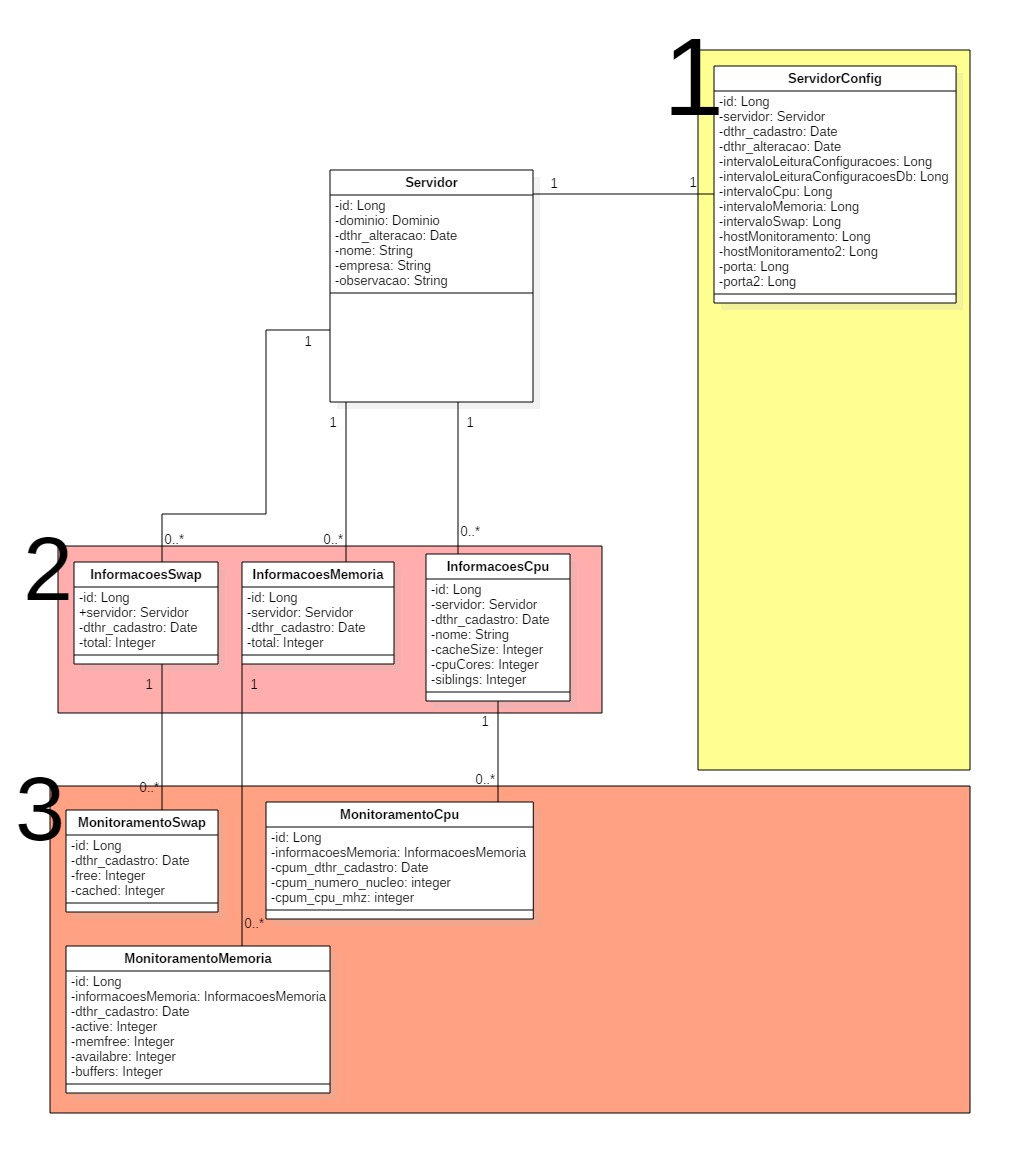
\includegraphics[width=1.0\textwidth]{figuras/DiagramaDeClass1.jpg}
	\caption[Diagrama de classe resumido 1.]{Diagrama de classe resumido 1, separados pelos grupos 1 à 3 que correspondem, respectivamente, às configurações que o usuário deve fazer, informações geradas pelo MonitorWeb-Cli e monitoramentos gerados pelo MonitorWeb-Cli}
	\label{Img:DiagramaDeClass1}
\end{figure}



\subsubsection{Classe ServidorConfig}
Como pode ser visto na \autoref{Img:DiagramaDeClass1}, a classe ServidorConfig possui um relacionamento de um-para-um com a classe Servidor, indicando assim que um objeto de Servidor pode ter somente um ServidorConfig. Essa classe é vital para o funcionamento do MonitorWeb-Cli. Dentro dela estão as configurações mínimas para que um MonitorWeb-Cli saiba como trabalhar. Na \autoref{Tab:VariaveisServidorConfig} explica-se detalhadamente a classe ServidorConfig.

Na \autoref{Tab:VariaveisServidorConfig}, o valor padrão das variáveis são apenas sugestões. O usuário pode alterar qualquer um deles, porém, é altamente recomendado que esses valores nunca sejam iguais a 0. Caso isso aconteça, o MonitorWeb-Cli enviará o máximo de informações que puder sem qualquer intervalo de tempo. Isso acaba consumindo o máximo de recurso (memória, cpu e disco) do sistema operacional hospedeiro.

\begin{table}[H]
\centering
\begin{tabular}{|l|l|}
\hline
{\color[HTML]{000000} \textbf{Variáveis}} & {\color[HTML]{000000} \textbf{Descriçães}} \\ \hline
id                                     & \multicolumn{1}{p{10.00cm}|}{Número único para cada objeto do tipo ServidorConfig. (Gerado Automaticamente)} \\ \hline
servidor                               & \multicolumn{1}{p{10.00cm}|}{Informa com qual servidor esse registro está relacionado.}
\\ \hline
dthr\_cadastro                         & \multicolumn{1}{p{10.00cm}|}{Data e hora do cadastro. (Gerado Automaticamente)}\\ \hline
dthr\_alteracao                        & \multicolumn{1}{p{10.00cm}|}{Data e hora que foi realizado a ultima alteração. (Gerado Automaticamente)(Essa funcionalidade não foi implementada)}\\ \hline
intervaloLeituraConfiguracoes          & \multicolumn{1}{p{10.00cm}|}{Intervalo em segundos para o MonitorWeb-Cli ler as configurações da classe ServidorConfig, e se reconfigurar(Valor padrão 120 s).} \\ \hline
intervaloLeituraConfiguracoesDb        & \multicolumn{1}{p{10.00cm}|}{Intervalo em segundos para o  MonitorWeb-Cli ler as configurações da classe ServidorConfigDb, e se reconfigurar(Valor padrão 120 s). Essa classe é mostrada na \autoref{subsubsec:ClasseServidorConfigDb}} \\ \hline
intervaloCpu                           & \multicolumn{1}{p{10.00cm}|}{Intervalo em segundos para o MonitorWeb-Cli enviar um registro da classe MonitoramentoCpu.(Valor padrão 1 s)}\\ \hline
intervaloMemoria                       & \multicolumn{1}{p{10.00cm}|}{Intervalo em segundos para o MonitorWeb-Cli enviar um registro da classe MonitoramentoMemoria.(Valor padrão 1 s)}\\ \hline
intervaloSwap                          & \multicolumn{1}{p{10.00cm}|}{Intervalo em segundos para o MonitorWeb-Cli enviar um registro da classe MonitoramentoSwap.(Valor padrão 1 s)} \\ \hline
hostMonitoramento                      & \multicolumn{1}{p{10.00cm}|}{IP que o MonitorWeb-Cli deve se comunicar.}\\ \hline
hostMonitoramento2                     & \multicolumn{1}{p{10.00cm}|}{IP secundário que o MonitorWeb-Cli deve se comunicar caso o servidor principal não esteja funcionando.(Essa funcionalidade não foi implementada)} \\ \hline
porta                                  & \multicolumn{1}{p{10.00cm}|}{Porta da aplicação para o MonitorWeb-Cli saber em que porta o MonitorWeb-Api está rodando.} \\ \hline
porta2                                 & \multicolumn{1}{p{10.00cm}|}{Porta da aplicação secundária para o MonitorWeb-Cli saber em que porta o MonitorWeb-Api está rodando.(Essa funcionalidade não foi implementada)} \\ \hline
\end{tabular}
\caption[Variáveis da classe ServidorConfig e suas descrições.]{Variáveis da classe ServidorConfig e suas descrições.}
\label{Tab:VariaveisServidorConfig}
\end{table}


\subsubsection{Classe ServidorConfigDb}\label{subsubsec:ClasseServidorConfigDb}

No diagrama de classe mostrado na \autoref{Img:DiagramaDeClass2} existem duas novas classes: a ServidorConfigDb no grupo um e a MonitoremantoPostgres no grupo três. Além das classes, um novo grupo número 4 é mostrado. Nesse grupo temos as \textit{enums} da aplicação, utilizadas em algumas classes.

\begin{figure}[H]
	\centering
	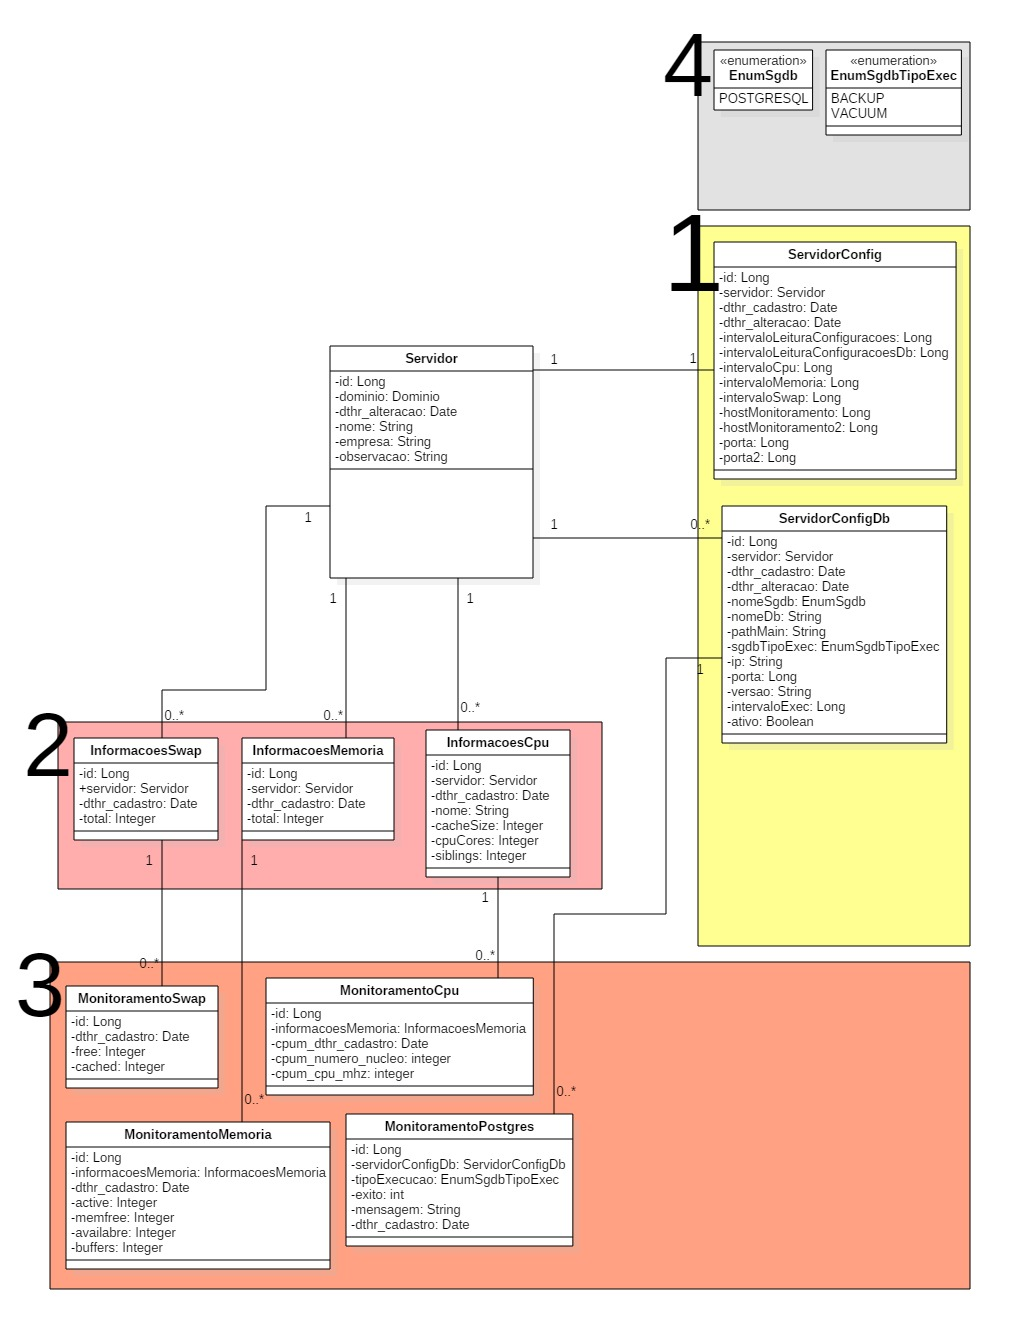
\includegraphics[width=1.0\textwidth]{figuras/DiagramaDeClass2.jpg}
	\caption[Diagrama de classe resumido 2.]{Diagrama de classe resumido 2, separados pelos grupos 1 à 4 que correspondem, respectivamente, às configurações que o usuário deve fazer, informações geradas pelo MonitorWeb-Cli, monitoramentos gerados pelo MonitorWeb-Cli e \textit{enums} da aplicação.}
	\label{Img:DiagramaDeClass2}
\end{figure}

A classe ServidorConfigDb é responsável por criar rotinas de \textit{backup} e \textit{vacuum} para o MonitoreWeb-Cli executar. Essa classe possui um relacionamento de muitos-para-um com a classe Servidor, o que indica que em um servidor pode ter diversas rotinas de \textit{backup} e \textit{vacuum}. Na \autoref{Tab:VariaveisServidorConfigDb} é explicada de forma minuciosa a classe ServidorConfigDb.

Essa classe também pode ser utilizada para o MonitoreWeb-Cli executar o procedimento de \textit{backup} e \textit{vacuum} em outro computador, para isso basta ser informado o IP da máquina que se deseja executar o procedimento e que a maquina esteja habilitada para fazer esse procedimento pela rede.

A classe MonitoremantoPostgres é responsável por armazenar os resultados dos \textit{backups} e dos procedimentos de \textit{vacuum} da classe ServidorConfigDb. A descrição de cada variável dessas classe pode ser vista no \autoref{App:ApendiceA}.

\begin{table}[H]
\centering
\begin{tabular}{|l|l|}
\hline
{\color[HTML]{000000} \textbf{Variável}} & {\color[HTML]{000000} \textbf{Descrição}}\\ \hline
id                                       & \multicolumn{1}{p{12.50cm}|}{Número único para cada objeto do tipo ServidorConfigDb. (Gerado Automaticamente) }\\ \hline
servidor                                 & \multicolumn{1}{p{12.50cm}|}{Indica com qual objeto Servidor esse registro está relacionado.}\\ \hline
dthr\_cadastro                           & \multicolumn{1}{p{12.50cm}|}{Data e hora do cadastro. (Gerado Automaticamente) } \\ \hline
dthr\_alteracao                          & \multicolumn{1}{p{12.50cm}|}{Data e hora que foi realizado a ultima alteração. (Gerado Automaticamente)}\\ \hline
nomeSgdb                                 & \multicolumn{1}{p{12.50cm}|}{É uma enum do tipo EnumSgdb, que informa em qual SGDB o procedimento será executado. Atualmente somente o postgreSQL é suportado. }\\ \hline
nomeDb                                   & \multicolumn{1}{p{12.50cm}|}{Nome do banco de dados que o procedimento será executado.}\\ \hline
pathMain                                 & \multicolumn{1}{p{12.50cm}|}{Caminho para as libs que executam o backup.}\\ \hline
sgdbTipoExec                             & \multicolumn{1}{p{12.50cm}|}{É uma enum do tipo EnumSgdbTipoExec o qual informa se o procedimento é um backup ou um vacuum.} \\ \hline
ip                                       & \multicolumn{1}{p{12.50cm}|}{IP para onde devera ser executado o procedimento. }\\ \hline
porta                                    & \multicolumn{1}{p{12.50cm}|}{Porta que será executado o procedimento. }\\ \hline
versao                                   & \multicolumn{1}{p{12.50cm}|}{Versão do SGDB.}\\ \hline
intervaloExec                            & \multicolumn{1}{p{12.50cm}|}{Intervalo de tempo que o MonitoreWeb-Cli deve executar esse procedimento.}\\ \hline
ativo                                    & \multicolumn{1}{p{12.50cm}|}{Controle para ativar e desativar o procedimento.}\\ \hline
\end{tabular}
\caption[Variáveis da classe ServidorConfigDb e suas descrições.]{Variáveis da classe ServidorConfigDb e suas descrições.}
\label{Tab:VariaveisServidorConfigDb}
\end{table}

\subsubsection{Classe ServidorConfigInformacoesDb}

No diagrama de classe mostrado na \autoref{Img:DiagramaDeClass3} existem duas novas classes: a ServidorConfigInformacoesDb no Grupo 1 e a MonitoremantoPostgresInformacoes no Grupo 3.

\begin{figure}[H]
	\centering
	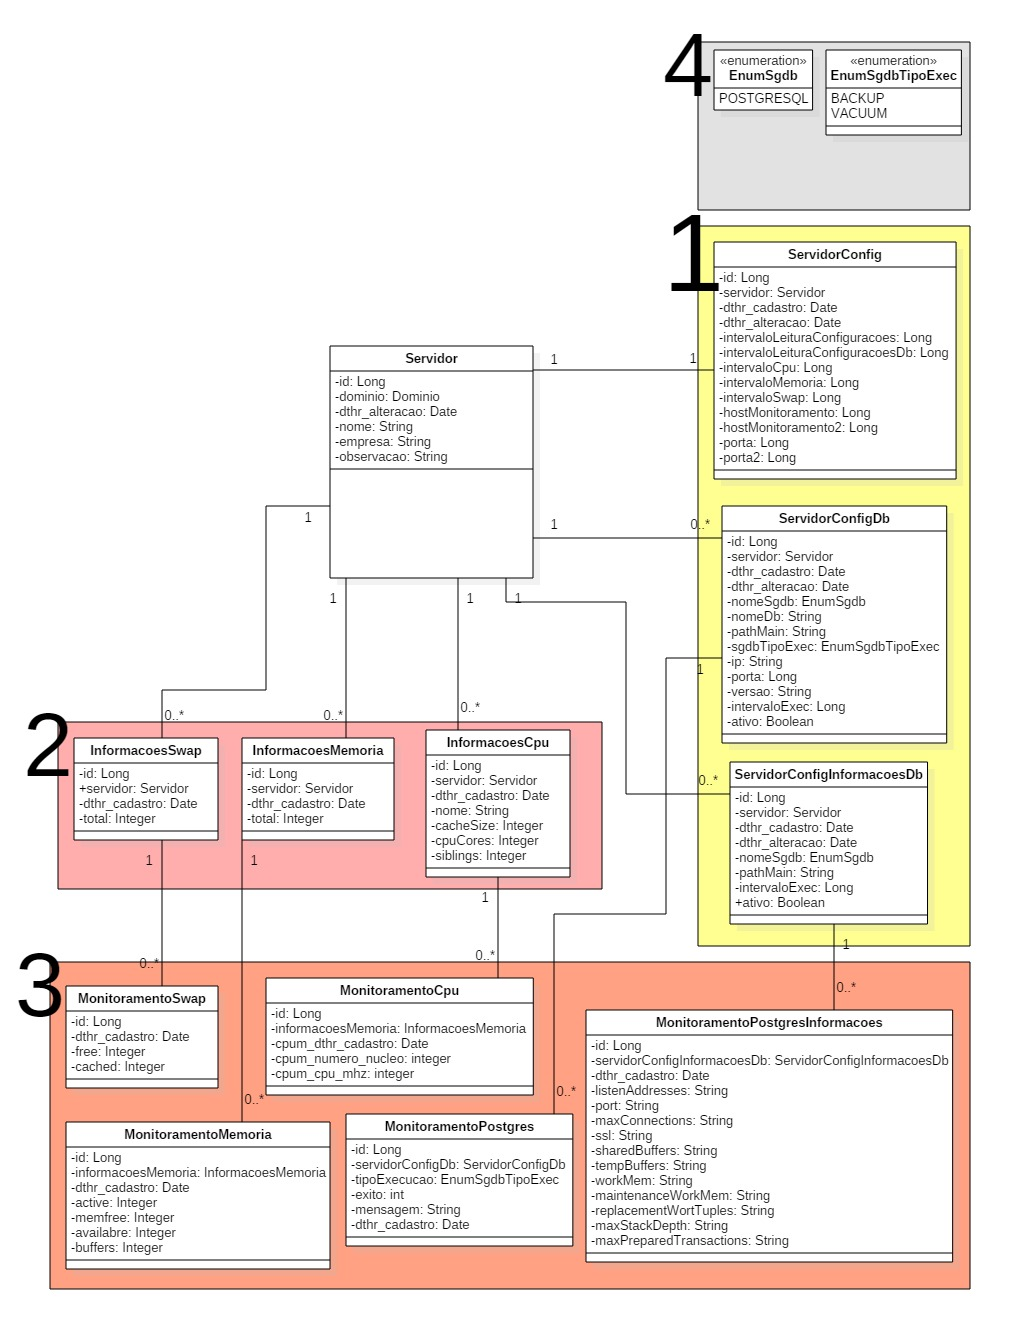
\includegraphics[width=1.0\textwidth]{figuras/DiagramaDeClass3.jpg}
	\caption[Diagrama de classe resumido 3.]{Diagrama de classe resumido 3, separados pelos grupos 1 à 4 que correspondem respectivamente a configurações que o usuário deve fazer, informações geradas pelo MonitorWeb-Cli, monitoramentos gerados pelo MonitorWeb-Cli e enums da aplicação.}
	\label{Img:DiagramaDeClass3}
\end{figure}

 A classe ServidorConfigInformacoesDb é responsável por criar uma rotina para ler o arquivo com as configurações principais do postgreSQL (postgresql.conf). Essa classe possui um relacionamento de muitos-para-um com a classe Servidor, uma vez que o servidor pode ter várias versões do banco de dados. Na \autoref{Tab:VariaveisServidorConfigInformacoesDb} descreve-se detalhadamente a classe ServidorConfigInformacoesDb.

A classe MonitoremantoPostgres é responsável por armazenar os resultados da classe ServidorConfigInformacoesDb. A descrição de cada variável da classe MonitoremantoPostgres pode ser vista no \autoref{App:ApendiceA}.


\begin{table}[H]
\centering
\begin{tabular}{|l|l|}
\hline
{\color[HTML]{000000} \textbf{Variável}} & {\color[HTML]{000000} \textbf{Descrição}}\\ \hline
id                                       & \multicolumn{1}{p{12.50cm}|}{Número único para cada objeto do tipo ServidorConfigDb. (Gerado Automaticamente)} \\ \hline
servidor                                 & \multicolumn{1}{p{12.50cm}|}{Indica com qual objeto Servidor esse registro está relacionado. }\\ \hline
dthr\_cadastro                           & \multicolumn{1}{p{12.50cm}|}{Data e hora do cadastro. (Gerado Automaticamente)}\\ \hline
dthr\_alteracao                          & \multicolumn{1}{p{12.50cm}|}{Data e hora que foi realizado a ultima alteração. (Gerado Automaticamente)}\\ \hline
nomeSgdb                                 & \multicolumn{1}{p{12.50cm}|}{É uma enum do tipo EnumSgdb, que informa em qual SGDB o procedimento será executado. Atualmente somente o postgreSQL é suportado. } \\ \hline
pathMain                                 & \multicolumn{1}{p{12.50cm}|}{Caminho para o arquivo postgresql.conf . }\\ \hline
intervaloExec                            & \multicolumn{1}{p{12.50cm}|}{Intervalo de tempo que o MonitoreWeb-Cli deve executar esse procedimento.} \\ \hline
ativo                                    & \multicolumn{1}{p{12.50cm}|}{Controle para ativar e desativar o procedimento. }\\ \hline
\end{tabular}
\caption[Variáveis da classe ServidorConfigInformacoesDb e suas descrições.]{Variáveis da classe ServidorConfigInformacoesDb e suas descrições.}
\label{Tab:VariaveisServidorConfigInformacoesDb}
\end{table}



\subsubsection{Diagrama de classe Usuários}\label{subsubsec:DiagramaClasseUsuarios}

No diagrama de classe mostrado na \autoref{Img:DiagramaDeClass4} existe um Grupo 5. Esse grupo está relacionado a um cadastro de usuário. Ele não é utilizado pelo MonitorWeb-Cli mas pode ser utilizado por implementações futuras para uma aplicação \textit{frontend} para o sistema. 

No Grupo 5 existem duas classes: a Usuario, que corresponde ao cadastro de contas de usuário na aplicação, e a Dominio, que corresponde a uma classe para dividir os usuários por grupo. Dessa forma, uma empresa que tenha diversos setores pode separar mais facilmente qual usuário tem acesso a qual grupo de servidores.

Além das duas classes, existe a classe UsuarioHasDominio que é simplesmente uma classe para uma ligação de muitos-para-muitos entre as classes Usuario e Dominio. A descrição de cada variável da classe Usuario e Dominio pode ser vistas no \autoref{App:ApendiceA}.
 
\begin{figure}[H]
	\centering
	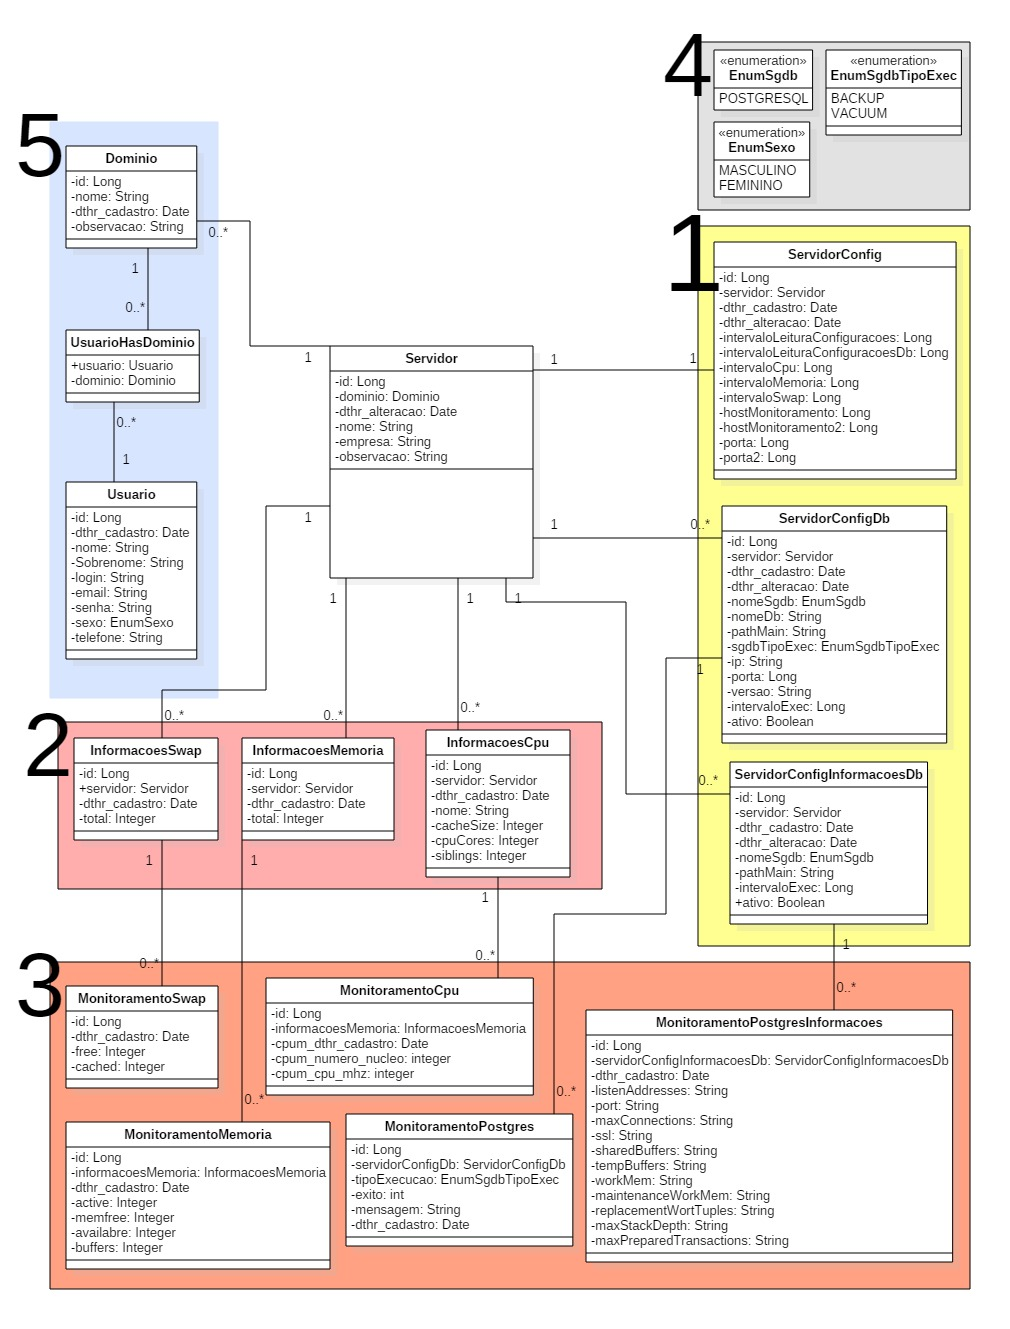
\includegraphics[width=1.0\textwidth]{figuras/DiagramaDeClass4.jpg}
	\caption[Diagrama de classe resumido 3.]{Diagrama de classe resumido 4, separados pelos grupos 1 à 5 que correspondem respectivamente a configurações que o usuário deve fazer, informações geradas pelo MonitorWeb-Cli, monitoramentos gerados pelo MonitorWeb-Cli, enums da aplicação e cadastro de usuários.}
	\label{Img:DiagramaDeClass4}
\end{figure}


\subsubsection{Diagrama de classe Completo}

No diagrama de classe mostrado na \autoref{Img:DiagramaDeClass} existe uma nova classe abstrata chamada de GenericEntity, sendo essa a superclasse para todas as entidades do sistema. A sua função é implementar os métodos \textit{equals} e \textit{hashCode} da classe Object. EXPLICAR O PORQUE!!! Além disso, ela cria os métodos abstratos getId, setId, getDthr\_cadastro e setDthr\_cadastro obrigando todos os métodos que estenderem dela a implementa-los.

A classe GenericEntity recebe um tipo T genérico que estende de Serializable. Esse tipo T representa o tipo da variável id da entidade, para que a aplicação saiba como gerar determinados métodos. A classe GenericEntity pode ser vista no \autoref{App:ApendiceB}.



\begin{figure}[H]
	\centering
	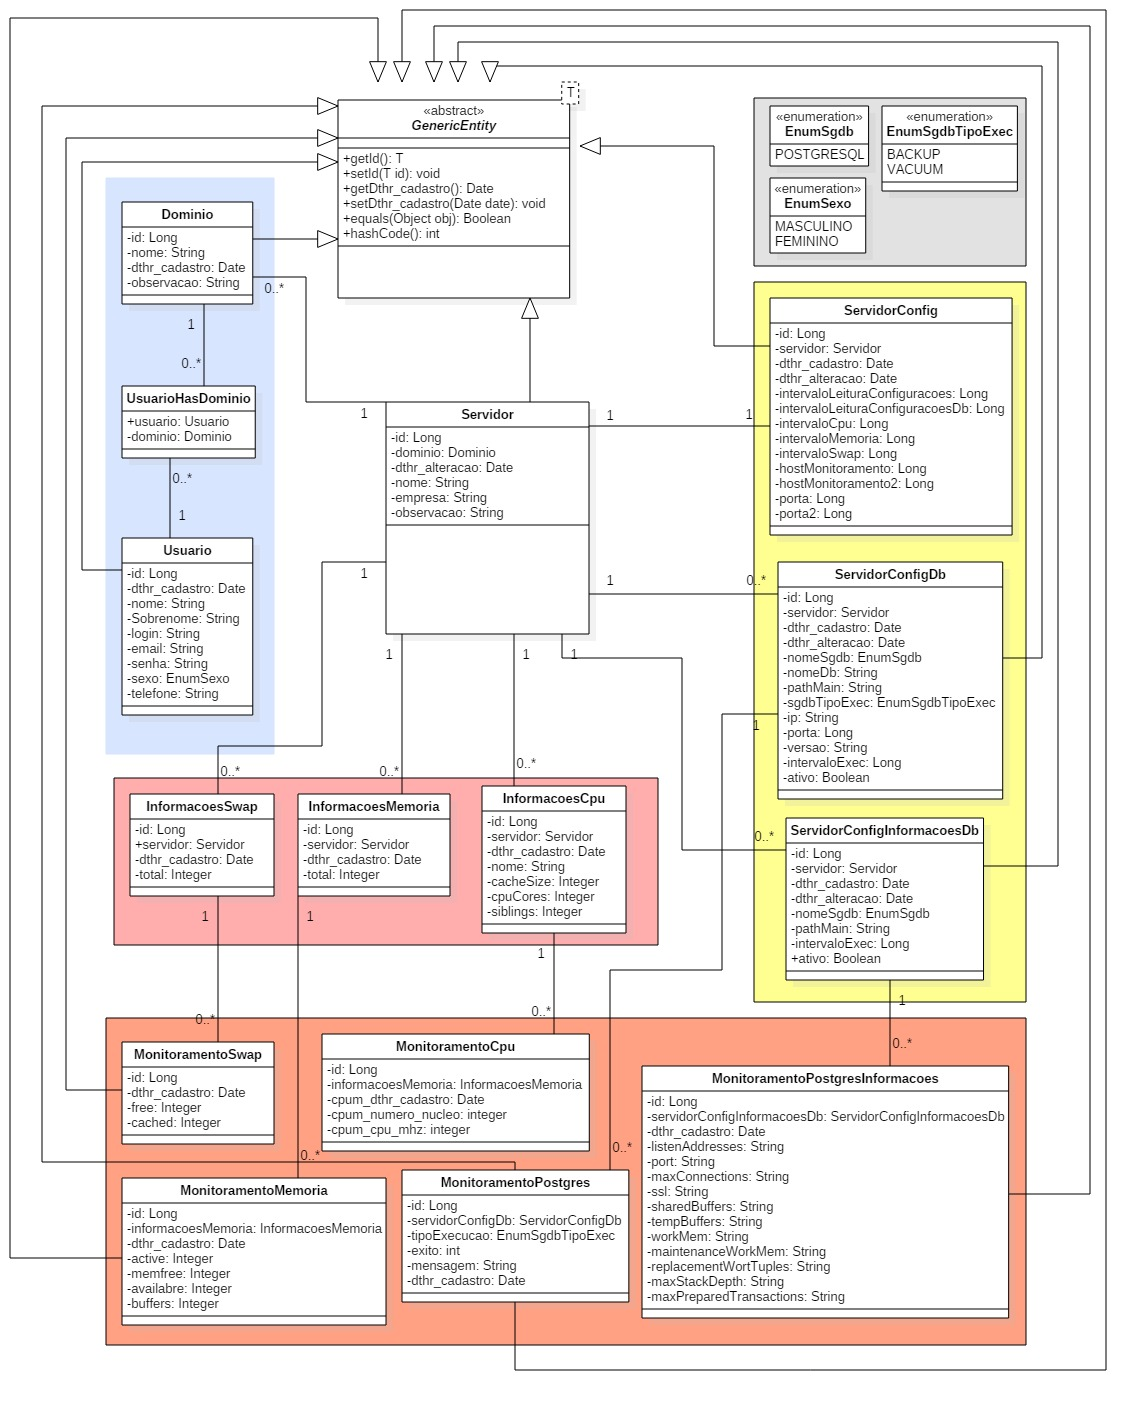
\includegraphics[width=1.0\textwidth]{figuras/DiagramaDeClass.jpg}
	\caption[Diagrama de classe completo.]{Diagrama de classe completo, separados pelos grupos 1 à 5 que correspondem respectivamente a configurações que o usuário deve fazer, informações geradas pelo MonitorWeb-Cli, monitoramentos gerados pelo MonitorWeb-Cli, enums da aplicação e cadastro de usuários.}
	\label{Img:DiagramaDeClass}
\end{figure}

\subsection{Configurações Apache Maven}\label{subsec:ConfiguraçõesApacheMaven}

Como visto na \autoref{sec:ApacheMaven} o Apache Maven é um gerenciador de pacotes responsável por gerir as dependências por meio do arquivo POM.
Esse arquivo é localizado na raiz do projeto (\url{/pom.xml}) e pode ser conferido no \autoref{App:ApendiceB}.

A seguir estão as principais dependências do projeto MonitorWeb-Api.

\begin{itemize}\label{List:Pom}
		\item \autoref{Func:POMMonitorWebApi}, linha 3 - spring-boot-starter-parent. Dependência do Spring Boot. Está dependência define uma versão base para que não seja necessário especificar as versões nos outros pacotes do Spring \cite{springBoot:2017}.
		
		\item \autoref{Func:POMMonitorWebApi}, linha 10 - spring-boot-starter-data-jpa. Dependência do Spring Data Jpa. Traz todas as dependências da JPA necessárias para o mapeamento das entidades \cite{springDataJpa:2017}.
		
		\item \autoref{Func:POMMonitorWebApi}, linha 15 - spring-boot-starter-web. Essa dependência identifica que a aplicação terá uma arquitetura \textit{web}, executando de forma embutida o servidor tomcat \cite{springBoot:2017}.
		
		\item \autoref{Func:POMMonitorWebApi}, linha 20 - spring-boot-starter-logging. Dependência responsável pelo registro de log automático \cite{springBoot:2017}.
		
		\item \autoref{Func:POMMonitorWebApi}, linha 25 - spring-boot-starter-test. Dependência do Spring Boot com bibliotecas de teste unitário, incluindo JUnit, Hamcrest e Mockito \cite{springBoot:2017}.
		
		\item \autoref{Func:POMMonitorWebApi}, linha 31 - postgresql, Dependência que fornece um conjunto padrão de interfaces para bancos de dados compatíveis com SQL \cite{PostgreSQL:2017}.
	
\end{itemize}


\begin{lstlisting}[style=XML,label=Func:POMMonitorWebApi,caption={[Arquivo POM com as principais dependências do projeto.]Arquivo POM com as principais dependências do projeto.}]
	<parent>
			<groupId>org.springframework.boot</groupId>
			<artifactId>spring-boot-starter-parent</artifactId>
			<version>1.3.3.RELEASE</version>
			<relativePath/>
	</parent>
	
	<dependency>
		<groupId>org.springframework.boot</groupId>
		<artifactId>spring-boot-starter-data-jpa</artifactId>
	</dependency>
	
	<dependency>
		<groupId>org.springframework.boot</groupId>
		<artifactId>spring-boot-starter-web</artifactId>
	</dependency>

	<dependency>
		<groupId>org.springframework.boot</groupId>
		<artifactId>spring-boot-starter-logging</artifactId>
	</dependency>

	<dependency>
		<groupId>org.springframework.boot</groupId>
		<artifactId>spring-boot-starter-test</artifactId>
		<scope>test</scope>
	</dependency>
				
	<dependency>
		<groupId>org.postgresql</groupId>
		<artifactId>postgresql</artifactId>
		<version>${postgresql.version}</version>
	</dependency>

	<dependency>
		<groupId>com.github.springtestdbunit</groupId>
		<artifactId>spring-test-dbunit</artifactId>
		<version>${spring-test-dbunit.version}</version>
		<scope>test</scope>
	</dependency>

	<dependency>
		<groupId>com.h2database</groupId>
		<artifactId>h2</artifactId>
		<scope>test</scope>
	</dependency>
\end{lstlisting}



\subsection{Configurações application.properties}\label{subsec:ConfiguraçõesApplicationProperties}

O Spring Boot fornece um arquivo de configuração com o nome de application.properties, e pode ser encontrado na pasta \url{/src/main/resources/application.properties}. Dentro desse arquivo pode ser feitas configurações de acordo com a necessidade do projeto \cite{springBoot:2017}. No \autoref{Func:applicationProperties} encontra-se o application.properties do MonitoreWeb-Api e a seguir uma lista contendo a descrição de cada configuração.

\begin{itemize}
		\item \autoref{Func:applicationProperties}, linha 2: server.port - Porta em que a aplicação será executada \cite{springBoot:2017}.
		
		\item \autoref{Func:applicationProperties}, linha 5: spring.jackson.date-format - Formato em que a data será apresentada \cite{springBoot:2017}.
		
		\item \autoref{Func:applicationProperties}, linha 10: logging.path - Indica o local do arquivo de \textit{log} \cite{springBoot:2017}.
		
		\item \autoref{Func:applicationProperties}, linha 19: spring.datasource.url - URL de conexão para o banco de dados \cite{springBoot:2017}.
		
		\item \autoref{Func:applicationProperties} linha 20: spring.datasource.username - Usuario do banco de dados \cite{springBoot:2017}.
		
		\item \autoref{Func:applicationProperties} linha 21: spring.datasource.password - Senha do banco de dados \cite{springBoot:2017}.
		
		\item \autoref{Func:applicationProperties} linha 22: spring.jpa.database-platform - Vários bancos de dados têm mais de um dialeto e essa propriedade especifica qual o hibernate irá utilizar \cite{springBoot:2017}.
		
		\item \autoref{Func:applicationProperties} linha 23: spring.datasource.driverClassName - Classe do \textit{driver} que será utilizado para conexão \cite{springBoot:2017}.
		
\end{itemize}

\begin{lstlisting}[style=LIVRE, label=Func:applicationProperties,caption={[Arquivo application.properties com as principais configurações do projeto.]Arquivo application.properties com as principais configurações do projeto.}]
## Portas
server.port=8081

## Formatador de datas do jackson
spring.jackson.date-format= yyyy-MM-dd'T'HH:mm:ss.SSSZ

## --------------------------------------------------------------------
## POSTGRES
## --------------------------------------------------------------------
spring.datasource.url=jdbc:postgresql://localhost/webmonitor
spring.datasource.username=postgres
spring.datasource.password=postgres
spring.jpa.database-platform=org.hibernate.dialect.PostgreSQLDialect
spring.datasource.driverClassName=org.postgresql.Driver

\end{lstlisting}


\subsection{Estrutura do Projeto}\label{subsec:EstruturaDoProjeto}

O projeto é dividido em seis pacotes Java que podem ser vistos na \autoref{Img:estruturaDePastaPojeto}, e uma classe na raiz com nome WebMonitorApp, a qual é responsável por iniciar a aplicação. Na \autoref{Tab:DescricaoDasPastasProjeto} apresenta-se a descrição de cada pacote.

\begin{figure}[H]
	\centering
	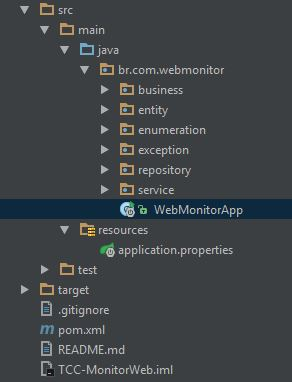
\includegraphics[width=0.5\textwidth]{figuras/estruturaPojeto.JPG}
	\caption[Estrutura dos pacotes Java do projeto.]{Estrutura dos pacotes Java do projeto.}
	\label{Img:estruturaDePastaPojeto}
	
	%width=0.5\textwidth (Tamanho da Imagem)
\end{figure}
	
% Please add the following required packages to your document preamble:
% \usepackage[table,xcdraw]{xcolor}
% If you use beamer only pass "xcolor=table" option, i.e. \documentclass[xcolor=table]{beamer}
\begin{table}[!ht]
\centering
\begin{tabular}{|l|l|}
\hline
\multicolumn{1}{|c|}{{\color[HTML]{000000} \textbf{Pasta}}} & {\color[HTML]{000000} \textbf{Descrição}} \\ \hline
business                                                    & \multicolumn{1}{p{10.00cm}|}{Responsável pelas regras de negocio. \autoref{subsubsec:business}. }\\ \hline
entity                                                      & \multicolumn{1}{p{10.00cm}|}{Contém as entidades do sistema. \autoref{subsec:DiagramaDeClasses}. }\\ \hline
enumeration                                                 & \multicolumn{1}{p{10.00cm}|}{Contém as enum da aplicação.}\\ \hline
exception                                                   & \multicolumn{1}{p{10.00cm}|}{Contém as exception da aplicação.}\\ \hline
repository                                                  & \multicolumn{1}{p{10.00cm}|}{Interfaces para gerar os acessos ao banco de dados. \autoref{subsubsec:Repository}.}\\ \hline
service                                                     & \multicolumn{1}{p{10.00cm}|}{Responsáveis pelos serviços da aplicação. \autoref{subsubsec:Service}.}\\ \hline
\end{tabular}
\caption{Descrição das pastas do projeto.}
\label{Tab:DescricaoDasPastasProjeto}
\end{table}


\subsubsection{Repository}\label{subsubsec:Repository}



O pacote repository Contém as interfaces de acesso ao banco de dados que são controladas pelo Spring Data. Todas essas interfaces devem herdar JpaRepository. Dessa forma, os métodos de consulta e persistência são gerados automaticamente pelo Spring Data.

Na \autoref{Img:estruturaDePastaRepository} pode ser visto que cada entidade da aplicação possui uma interface repository. O padrão de nomenclatura utilizado nas interfaces é: <nome-da-entidade> seguido pela palavra "Repository".

\begin{figure}[H]
	\centering
	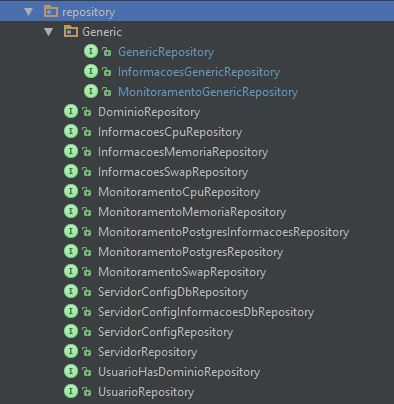
\includegraphics[width=0.5\textwidth]{figuras/estruturaPojetoRepository.JPG}
	\caption[Pasta Repository.]{Pasta Repository.}
	\label{Img:estruturaDePastaRepository}
\end{figure}


\subsubsection{Business}\label{subsubsec:business}

A pasta business é responsável pelas regras de negocio da aplicação. Cada entidade contém uma classe business correspondente que segue o padrão de nomenclatura: <nome-da-entidade> mais "BO", como pode ser visto na \autoref{Img:estruturaDePastaBusiness}. 

Todas as classes da business herdam a classe GenericBO que Contém os métodos genéricos de inserção e exclusão do banco de dados. 

A GenericBO recebe dois parâmetros: o primeiro, um tipo genérico Entity que deve ser herdado da classe GenericEntity; o segundo, uma classe Repository que tenha implementado a interface JpaRepository para a respectiva entidade, o que informa que essa classe possui um repositório de acesso ao banco de dados controlado pelo Spring Boot. A classe GenericBO pode ser vista no \autoref{App:ApendiceB}.

\begin{figure}[H]
	\centering
	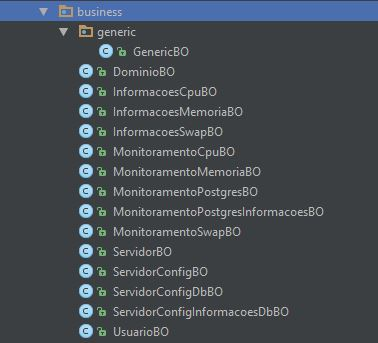
\includegraphics[width=0.5\textwidth]{figuras/estruturaPojetoBusines.JPG}
	\caption[Pasta Business.]{Pasta Business.}
	\label{Img:estruturaDePastaBusiness}
\end{figure}



\subsubsection{Service}\label{subsubsec:Service}

As classes da pasta service são as responsáveis por receber as requisições HTTP e responde-las de acordo com a especificação da arquitetura ReST. Cada entidade da aplicação contém uma classe Service correspondente que segue o padrão de nomenclatura: <nome-da entidade> seguido da palavra "Service", como pode ser visto na \autoref{Img:estruturaDePastaService}.

Cada classe possui uma URL destinada a gerenciar seus recursos. Essas URLs aceitam os métodos GET, POST e DELETE que correspondem, respectivamente, à listagem, inserção e remoção de um recurso. Na \autoref{Tab:UrlRecursos} mostra-se essas URLs, e na \autoref{subsec:ConsumindoRecursos} está explicado como utiliza-las.


- - - - - - - - - - - - - - - - - - - - - - - - - - - - - - - - - - - - - - - - - - - - - - - - - - - - - - - - - - - - 
- - - - - - - - - - - - - - - - - - - - - - - - - - - - - - - - - - - - - - - - - - - - - - - - - - - - - - - - - - - - 
- - - - - - - - - - - - - - - - - - - - Kleber continuar a revisão daqui - - - - - - - - - - - - - - - - - - - - - - - -
- - - - - - - - - - - - - - - - - - - - - - - - - - - - - - - - - - - - - - - - - - - - - - - - - - - - - - - - - - - - 
- - - - - - - - - - - - - - - - - - - - - - - - - - - - - - - - - - - - - - - - - - - - - - - - - - - - - - - - - - - - 
- - - - - - - - - - - - - - - - - - - - - - - - - - - - - - - - - - - - - - - - - - - - - - - - - - - - - - - - - - - - 


Na \autoref{Tab:UrlRecursos} os valores entre chaves representam o id do objeto a qual o recurso está relacionado. Por exemplo, na URL \url{/servidor/{idServidor}/informacoescpu}, o valor \{idServidor\} representa o id do Servidor a qual o objeto da classe InformacoesCpu está relacionado. Dessa forma essa requisição traz todos os objetos de InformacoesCpu relacionados com o Servidor de número \{idServidor\}.



\begin{figure}[H]
	\centering
	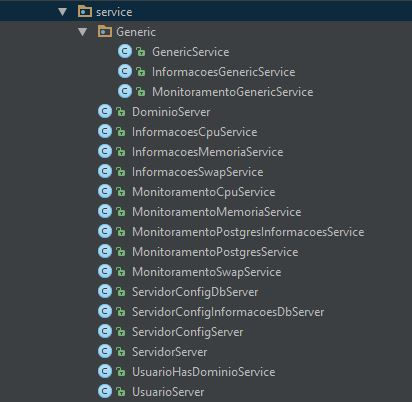
\includegraphics[width=0.5\textwidth]{figuras/estruturaPojetoService.JPG}
	\caption[Pasta Service.]{Pasta Service.}
	\label{Img:estruturaDePastaService}
\end{figure}


\begin{table}[H]
\centering
\begin{tabular}{|l|l|}
\hline
{\color[HTML]{000000} \textbf{Classe}}  & {\color[HTML]{000000} \textbf{URL}} \\ \hline
Usuario                           & \multicolumn{1}{p{9.00cm}|}{\url{/usuario }} \\ \hline
Dominio                           & \multicolumn{1}{p{9.00cm}|}{\url{/dominio }}  \\ \hline
Servidor                          & \multicolumn{1}{p{9.00cm}|}{\url{/servidor }}  \\ \hline
InformacoesCpu                   & \multicolumn{1}{p{9.00cm}|}{\url{/servidor/{idServidor}/informacoescpu}}   \\ \hline
InformacoesMemoria               & \multicolumn{1}{p{9.00cm}|}{\url{/servidor/{idServidor}/informacoesmemoria}}  \\ \hline
InformacoesSwap                  & \multicolumn{1}{p{9.00cm}|}{\url{/servidor/{idServidor}/informacoesswap }} \\ \hline
MonitoramentoCpu                 & \multicolumn{1}{p{9.00cm}|}{\url{/servidor/informacoes/{idInformacoesCpu}/monitoramentocpu}}\\ \hline
MonitoramentoMemoria             & \multicolumn{1}{p{9.00cm}|}{\url{/servidor/informacoes/{idInformacoesMemoria}/monitoramentomemoria}}\\ \hline
MonitoramentoPostgresInformacoes & \multicolumn{1}{p{9.00cm}|}{\url{/servidor/informacoes/{idInformacoesPostgresInformacoes}/monitoramentopostgresinformacoes}}\\ \hline
MonitoramentoPostgres            & \multicolumn{1}{p{9.00cm}|}{\url{/servidor/informacoes/{idInformacoesPostgres}/monitoramentopostgres}} \\ \hline
MonitoramentoSwap                & \multicolumn{1}{p{9.00cm}|}{\url{/servidor/informacoes/{idInformacoesSwap}/monitoramentoswap }}  \\  \hline
ServidorConfigDb                 & \multicolumn{1}{p{9.00cm}|}{\url{/servidor/{idServidor}/servidorconfiguracoesdb }}\\ \hline
ServidorConfigInformacoesDb      & \multicolumn{1}{p{9.00cm}|}{\url{/servidor/{idServidor}/servidorconfiguracoesinformacoesdb }}  \\  \hline
ServidorConfig                   & \multicolumn{1}{p{9.00cm}|}{\url{/servidor/{idServidor}/servidorconfiguracoes }}\\ \hline
\end{tabular}
\caption[URLs da aplicação MonitorWeb-Api.]{URLs da aplicação MonitorWeb-Api. }
\label{Tab:UrlRecursos}
\end{table}


\subsection{Consumindo recursos do MonitorWeb-Api}\label{subsec:ConsumindoRecursos}

Os recursos do MonitorWeb-Api são consumidos utilizando o protocolo HTTP. Nas subseção a seguir será mostrado como utilizar os recursos da aplicação.

Todos os exemplos a seguir supõem que o MonitorWeb-Api esteja rodando no ip 127.0.0.1 e utilizando a porta 8081. 

\subsubsection{Get}



\begin{lstlisting}[label=Func:GETExemplo,caption={[].}]
GET /servidor HTTP/1.1
Host: 127.0.0.1:8081
Accept: application/json
\end{lstlisting}


\begin{lstlisting}[label=Func:RespostaExemplo,caption={[]}]
HTTP/1.1 200 OK
Content-Type: plication/json
Content-Length: 316
{
    "id": 1,
    "dominio": {
        "id": 1,
        "nome": "Nome do Dominio",
        "dthr_cadastro": "2017-01-01T03:00:00.000+0000",
        "observacao": "Observação do Dominio"
    },
    "dthr_cadastro": "2017-01-02T03:00:00.000+0000",
    "nome": "Nome do Servidor",
    "empresa": "empresa 1",
    "observacao": "OBS"
}
\end{lstlisting}

%# # # # # # # # # # # # # # # # # # # # # # # # # # # # # # # # # # # # # # # # # # # # # # # # # # # # # # # # # # # # # # # # # # # # # # # # # # # # # # # # # # # # # # # # # # # # # # # # # # # # # # # # # # # # # # # # # # # # # # # # # # # # # # # # # # # # # # # # # # # # # # # # # # # # # # # # # # # # # # # # # # # # # # # # # # # # # # # # # # # # # # # # # # # # # # # # # # # # # # # # # # # # # # # # # # # # # # # # # # # # # # # # # # # # # # # # # # # # # # # # # # # # # # # # # # # # # # # # # # # # # # # # # # # # # # # # # # # # # # # # # # # # # # # # # # # # # # # # # # # # # # # # # # # # # # # # # # # # # # # # # # # # # # # # # # # # # # # # # # # # # # # # # # # # # # # # # # # # # # # # # # # # # # # # # # # # # # # # # # # # # # # # # # # # # # # # # # # # # # # # # # # # # # # # # # # # # # # # # # # # # # # # # # # # # # # # # # # # # # # # # # # # # # # # # # # # # # # # # # # # # # # # # # # # # # # # # # # # # # # # # # # # # # # # # # # # # # # # # 


\section{MonitorWeb-Cli}\label{sec:MonitorWeb-Cli}

\begin{figure}[H]
	\centering
	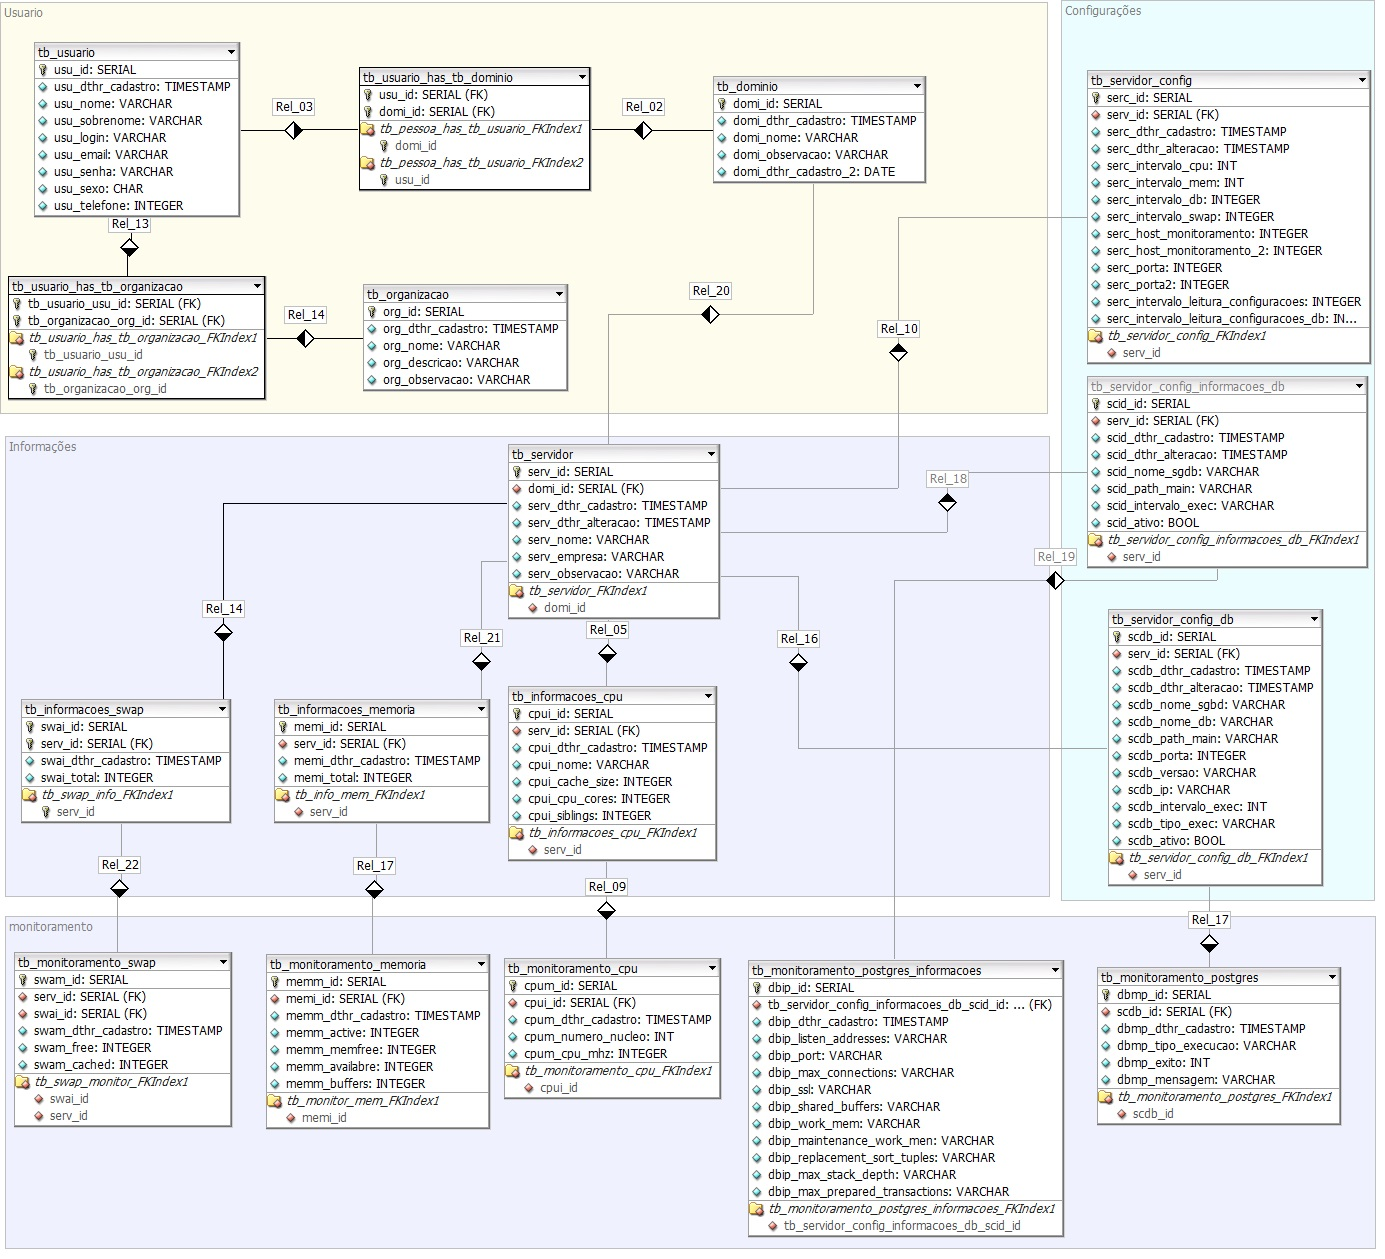
\includegraphics[width=1.0\textwidth]{figuras/diagramaBanco.jpg}
	\caption[Pasta Entitybbbbbbbbbbbbbbbbbbbbbbbbbbbbbbbbbb.]{Pasta Entityaaaaaaaaaaaaaaaaaaaaaaaaaaaaaaaaaaaa.}
	\label{Img:estruturaDePastaPojetoEntity}
	
	%width=0.5\textwidth (Tamanho da Imagem)
\end{figure}


